\section{Our Approach}
\begin{frame}{Our Approach}
    \begin{description}
    \item[\acs{approachname}] \acl{approachname}
    \end{description}
    
    \only<1>{
        \begin{figure}[htbp]
        \centering
            \includegraphics[height=0.6\textheight]{images/DALLE_2025_02_21_fat_cat.png}
        \label{fig:fat_cat}
    \end{figure}
    Image generated by DALLE (February 21, 2025)
    }

    \only<2->{
        \begin{figure}[htbp]
        \centering
        \scalebox{0.9}{
            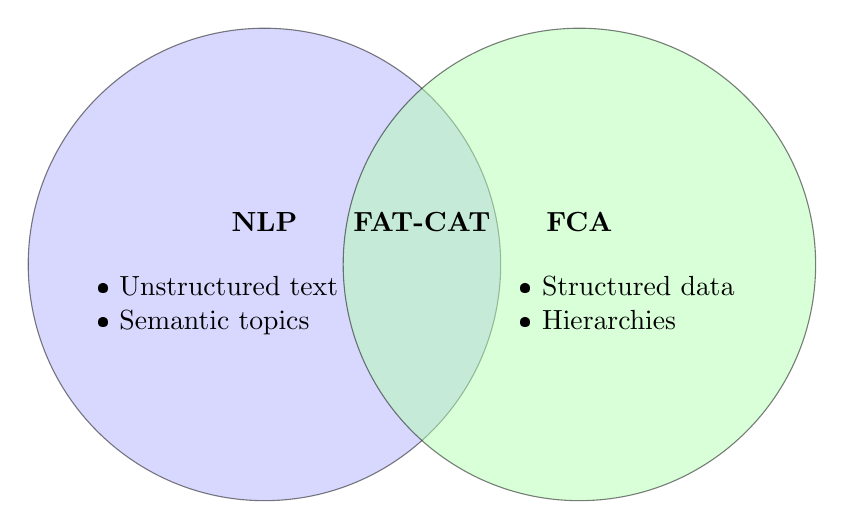
\begin{tikzpicture}
                 % Draw circles
                \draw[fill=blue!30, opacity=0.5] (-2,0) circle (3);
                \draw[fill=green!30, opacity=0.5] (2,0) circle (3);

                % Labels above circles
                \node[above] at (-2,0.3) {\textbf{NLP}};
                \node[above] at (2,0.3) {\textbf{FCA}};
                \node[above] at (0,0.3) {\textbf{FAT-CAT}};

                % NLP-only contributions (inside left circle, lower)
                \node[align=left] at (-2.6,-0.7) {
                    \textbullet\ Unstructured text\\
                    \textbullet\ Semantic topics\\
                    % \textbullet\ Statistical\\
                };

                % FCA-only contributions (inside right circle, lower)
                \node[align=left] at (2.6,-0.7) {
                    \textbullet\ Structured data\\
                    \textbullet\ Hierarchies\\
                    % \textbullet\ Deductive reasoning\\
                };
            \end{tikzpicture}
        }
        \label{fig:venn_nlp_fca}
    \end{figure}
    }

\end{frame}

\begin{frame}{Our Approach}
    \begin{description}
    \item[\acs{approachname}] \acl{approachname}
    \end{description}

    Our contributions:
    \begin{itemize}
        \uncover<2->{\item Open-source\footnote{\url{https://github.com/KlaraGtknst/text_topic} (29.01.2025) \&\\ \url{https://github.com/KlaraGtknst/clj_exploration_leaks} (29.01.2025)}}
        \uncover<3->{\item Minimal training requirements}
        \uncover<4->{\item Non-textual data} % \item[\rightarrowfill]
        \uncover<5->{\item Information aggregation across directories}       
    \end{itemize}
\end{frame}

\begin{frame}{Text Extraction}
    \includesvg[width=\linewidth]{images/extract_text}
    \label{fig:extract_text}
    \begin{beamercolorbox}[center, wd=\linewidth, sep=1ex, rounded=true, shadow=true]{block body}
        {\small Appendix details: } 
        \hyperlink{supp:img_cap}{\beamergotobutton{Image Captioner}}
    \end{beamercolorbox}
\end{frame}


\begin{frame}{Text Processing}
    \includesvg[width=\linewidth]{images/text_related_workflow}
      \vfill
    \begin{beamercolorbox}[center, wd=\linewidth, sep=1ex, rounded=true, shadow=true]{block body}
        {\small Appendix details: } 
        \hyperlink{supp:img_cap}{\beamergotobutton{Image Captioner}}
        \hspace{1em}
        \hyperlink{supp:sbert}{\beamergotobutton{SBERT}}
    \end{beamercolorbox}
\end{frame}

